\section{Evaluation}
\label{sec:eval}

\paragraph{Setup (shared).} Seven \texttt{trn1.32xlarge} instances
in a single AWS Virtual Private Cloud (VPC), with Elastic Fabric
Adapter (EFA) networking enabled. Each node has 32 NeuronCores
(the per-chip compute tiles on Trainium); the cluster totals 224
ranks. Cross-node bandwidth comes from 8 EFA adapters per node at
12.5~GB/s each. We run all measurements with
\texttt{NEURON\_NUM\_RECENT\_MODELS\_TO\_KEEP=1}, the standard
production setting for large-LLM training on Trainium: each
\texttt{mark\_step} pair compiles a fresh HLO graph, and the
device-side NEFF
cache cannot grow without bound, so keeping only the
single-most-recently-used NEFF resident is the practitioner default
to bound HBM (high-bandwidth memory) scratchpad and DMA-ring
(direct-memory-access transfer) allocations. It is also the regime
in which any NEFF-cache-pressure effects on the candidate
strategies become visible. LLM: Claude Sonnet~4.5 (used as
mutation oracle in Phase~3). The baseline is the
internal-AWS-optimized strategy used in production for
large-MoE and dense-transformer Trainium training
(Section~\ref{sec:model}).

\subsection{General setup, methodology, and search cost}
\label{sec:eval-general}

Before the OLMoE and Llama harness-specific subsections, this
subsection presents items that apply uniformly to both: the
evaluation harness layout, the measurement methodology (late-phase
probe, per-call across scopes), the cross-scope finding that
motivates running training at all, and the search cost incurred
once across the eight collective problems. Table~\ref{tab:setup}
summarizes the two harness types we use throughout this section ---
a per-problem microbench that wraps a single collective in a small
MoE-shaped training step, and end-to-end training scripts that
drive the full forward$+$backward pass with all relevant
collectives composed.

\begin{table*}[h]
\centering\small
\setlength{\tabcolsep}{4pt}
\begin{tabular}{lll}
\toprule
 & \textbf{Per-problem microbench} & \textbf{End-to-end} \\
\midrule
Scale, steps     & 1 node $\cdot$ 32 ranks, 5000          & 7 nodes $\cdot$ 224 ranks, 250 \\
Model shell      & DeepSeek-MoE-Lite-shaped   & OLMoE-architectural-style \\
\textsc{layers/dm/heads}    & 12 / 2048 / 16  & 8 / 2048 / 16 \\
\textsc{nexp/topk/exdim}    & 64 / 6 / 1408             & 224 ($=\!\text{ws}$) / 8 / 1024 \\
\textsc{seqlen/bsz/vocab}   & 256 / 1 / 32768 & 256 / 1 / 32256 (sharded) \\
Routing          & token-choice top-K          & expert-choice (exp=1.0, cap=10) \\
Collective under test & one per script         & AllToAllV $+$ dxe \\
\bottomrule
\end{tabular}
\caption{Setup of the two evaluation harnesses, bf16 with full
autograd backward.}
\label{tab:setup}
\end{table*}

\paragraph{Per-call timings across scopes.} Table~\ref{tab:perproblem}
measures each problem's central collective at three
progressively wider scopes: \textbf{1-node bench}, the standard
small-scale microbenchmark practitioners run --- the collective
is called in isolation, 20 times in a tight loop, on the
NeuronLink interconnect alone, at 32 ranks (a single Trainium
node); \textbf{7-node bench}, the same idea but at the
production scale of 224 ranks across 7 nodes, where the EFA
network now mediates cross-node traffic; and \textbf{7-node
training}, the per-step cost of the collective as measured
\emph{from inside a real training step}, by reading the elapsed
time of the call within the autograd function that wraps it.
The 1-node bench is the cheapest and closest to what a
microbenchmark exercises; the 7-node training column is the
ground truth we care about.

\begin{table*}[t]
\centering\small
\setlength{\tabcolsep}{4pt}
\begin{tabular}{lrrrrrr}
\toprule
\textbf{Problem} & \multicolumn{2}{c}{\textbf{1-node bench (ms/call)}} & \multicolumn{2}{c}{\textbf{7-node bench (ms/call)}} & \multicolumn{2}{c}{\textbf{7-node training (ms/step)}} \\
                 & \textbf{baseline} & \textbf{agent} & \textbf{baseline} & \textbf{agent} & \textbf{baseline} & \textbf{agent} \\
\midrule
\multicolumn{7}{l}{\textit{OLMoE collectives}} \\
AllToAllV       & \textbf{1.83} & 1.95 & \textbf{1.89} & 3.04 & 4410 & \textbf{3352} \\
Uniform A2A     & \textbf{46.95} & 47.87 & 55.4 & \textbf{52.3} & 373.2 & \textbf{206.2} \\
Ring KV         & 3.57 & \textbf{1.07} & 2.95 & \textbf{2.02} & 13.49 & \textbf{10.32} \\
dxe (dist.\ CE) & 1.64 & \textbf{0.37} & 1.87 & \textbf{0.57} & 16.74 & \textbf{14.63} \\
\midrule
\multicolumn{7}{l}{\textit{Llama primitives (per-step contribution from amp1 probe)}} \\
PP cross-stage  & \textbf{1.78} & 2.38 & \textbf{1.34} & 2.37 & 21.36 & \textbf{4.11} \\
TP MLP          & \textbf{1.91} & 2.83 & \textbf{0.64} & 1.67 & 8.04 & \textbf{1.93} \\
FSDP prefetch   & \textbf{1.21} & 2.00 & 1.37 & \textbf{1.39} & 8.52 & \textbf{2.01} \\
Layer-block AR  & \textbf{0.89} & 2.94 & \textbf{1.15} & 4.35 & 9.40 & \textbf{2.26} \\
\bottomrule
\end{tabular}
\caption{Three measurement scopes per primitive: 1-node 32-rank bench, 7-node 224-rank bench, and 7-node
per-step contribution at training scope. Bold marks the faster of each (baseline, agent) pair.}
\label{tab:perproblem}
\end{table*}

\begin{table*}[t]
\centering\small
\setlength{\tabcolsep}{5pt}
\begin{tabular}{llrrrr}
\toprule
\textbf{Harness} & \textbf{Backend} & \textbf{Wall (min)} & \textbf{Steady (ms)} & \textbf{Final loss} & \textbf{Speedup} \\
\midrule
\multirow{2}{*}{\textit{OLMoE-10B}}
  & baseline (developer)            & 183.6 & 4407.4 & 6.843 & 1.000$\times$ \\
  & agent (strategy-enumerate)      & 130.2 & 3125.8 & 6.945 & $\mathbf{1.41\times}$ \\
\midrule
\multirow{2}{*}{\textit{Llama-7B}}
  & baseline (per\_mb, developer)   & 2.5 & 71.3 & 4.970 & 1.000$\times$ \\
  & agent (strategy-enumerate)      & 5.9 & 22.0 & 4.970 & $\mathbf{3.24\times}$ \\
\bottomrule
\end{tabular}
\caption{End-to-end speedups of strategy-enumerate over the developer baseline. OLMoE-10B:
ws=224, \emph{2500 steps with real OpenWebText, AdamW $\text{lr}_{\max}{=}5\!\times\!10^{-4}$
cosine, warmup 200}, bf16, AllToAllV$+$DXE; both backends descend from log~V$\approx$10.4 to
final loss in the 6.8--7.0 range (loss-curve plot in Figure~\ref{fig:loss-curve}), with
trajectory bit-identical or within $\pm$0.15 at every checkpoint (algorithm-equivalence). Llama-7B:
ws=224, 200 steps, bf16, PP$+$TP MLP$+$FSDP$+$lbar; final loss bit-identical at the precision
reported (random-token training, algorithm-equivalence proof). A short pretraining-slice loss-curve
match is in §\ref{sec:loss-match}. Matching cc-react / multi-island ablations are in
Table~\ref{tab:ablation-e2e}.}
\label{tab:e2e}
\end{table*}

\paragraph{Headline result.} Table~\ref{tab:e2e} is the
load-bearing result: $1.41\times$ end-to-end on OLMoE-10B and
$3.24\times$ end-to-end on Llama-7B over an
internal-AWS-optimized baseline used in production for large
MoE and dense transformer training, with algorithm-equivalent
descent (real OpenWebText for OLMoE,
Figure~\ref{fig:loss-curve}; random-token for Llama-7B,
bit-identical per-microbatch-normalized loss). The per-call/per-step
destrategy that shows why is in Figure~\ref{fig:disagree}.

\begin{figure*}[!htbp]
\centering
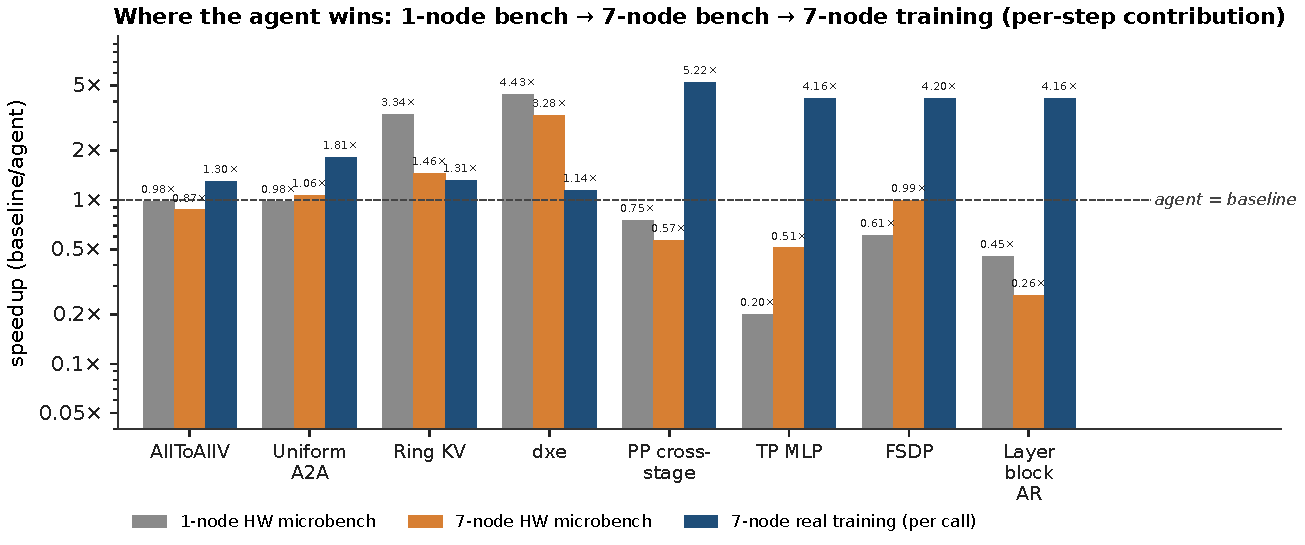
\includegraphics[width=0.85\linewidth]{figures/disagreement.pdf}
\caption{\textbf{Cross-scope inversion --- the core empirical
finding.} Per-problem speedup (baseline$/$agent) at three
measurement scopes: 1-node bench, 7-node bench, and 7-node
per-step contribution at training scope. Bars are computed
from the strategy-enumerate reference numbers in
Table~\ref{tab:perproblem}; dashed line marks agent$=$baseline.
For the majority of primitives, the per-call ranking at the
bench scopes practitioners actually calibrate against (left two
bars) is inverted at training scope (right bar) --- the agent
strategy that loses or ties per call wins $4$--$5\times$ at
training scale on the Llama primitives. Ring KV and dxe are
exceptions: the agent already wins at the 1-node bench on
those, so the cross-scope effect amplifies an existing advantage
rather than reversing one. This is the per-primitive mechanism
behind the $1.41\times$ OLMoE and $3.24\times$ Llama end-to-end
speedups (Table~\ref{tab:e2e}); see §\ref{sec:eval-llama} for
the Llama-side discussion.}
\label{fig:disagree}
\end{figure*}

\iffalse % Table 4 merged into Table~\ref{tab:perproblem} above
\begin{table}[h]
\centering\small
\setlength{\tabcolsep}{3pt}
\begin{tabular}{lrrrrrrr}
\toprule
\textbf{Problem} & \multicolumn{2}{c}{\textbf{1-node bench/call}} & \multicolumn{2}{c}{\textbf{7-node bench/call}} & \multicolumn{2}{c}{\textbf{7-node training/call}} & \textbf{Trend} \\
& base & agent & base & agent & base & agent & \\
\midrule
AllToAllV & 1.66 & 2.75 & ---$^{\,*}$ & 3.88 & $\sim$135$^{\,\dagger}$ & $\sim$95$^{\,\dagger}$ & flip in training \\
Uniform A2A & 8.63 & 3.67 & ---$^{\,*}$ & 0.26 & 86.62 & 66.15 & 2.35$\to$1.31$\times$ \\
Ring KV & 4.73 & 0.87 & 2.80 & 1.57 & 25.99 & 24.12 & 5.43$\to$1.78$\to$1.08$\times$ \\
dxe & 1.25 & 7.29 & 0.95 & 9.22 & 11.2 & 9.0 & loses isolated 0.17/0.10$\times$, wins in train 1.24$\times$ \\
\bottomrule
\end{tabular}
\caption{Per-call hardware time, in ms, at three measurement
scopes for the four collectives. \textbf{1-node bench/call}: isolated
20-iter HW microbench, 32 ranks, NeuronLink only. \textbf{7-node
bench/call}: isolated 30-iter HW microbench, 224 ranks, NeuronLink
$+$ EFA (\texttt{experiments/h7\_bench/}). \textbf{7-node
training/call}: 800-sample mean (idx$\geq$200 of 1000 steps)
measured via an \texttt{.item()} probe inside the autograd
\texttt{Function}'s \texttt{forward}/\texttt{backward}. The
three scopes give different ratios for the same strategy:
the agent's win shrinks as we move from isolated 1-node $\to$
isolated 7-node $\to$ real training, because Neuron fuses adjacent
\texttt{xm.*} calls inside a single \texttt{mark\_step} graph and
real training has many such graphs back to back. \textsuperscript{$*$}The
AG$+$RS baseline runs cleanly inside the training scripts but hits
an XLA trace-time shape-inference issue when called in isolation
(\texttt{xm.all\_gather} on an \texttt{unsqueeze(0)} reports
\texttt{(1, N)} at trace, breaks the subsequent
\texttt{view(ws, ws, mc)}); we report the agent-only 7-node
isolated number until the bench infra is unblocked.
\textsuperscript{$\dagger$}Estimated from the OLMoE fwd/bwd phase
destrategy. \textsuperscript{$\ddagger$}From the ce phase of the
OLMoE 7-node run, where dxe replaces a $(B \cdot S, V)$ all-gather
with two small AR.}
\label{tab:percall_real}
\end{table}
\fi % end of commented-out merged table

\subsection{OLMoE end-to-end training}
\label{sec:eval-olmoe}

The OLMoE end-to-end harness drives a transformer with the same
architecture as OLMoE~\cite{muennighoff2024olmoe}: multi-head
attention with rotary position embeddings
(RoPE,~\cite{su2024roformer}) and RMSNorm
normalization~\cite{zhang2019rmsnorm}, followed by a
Mixture-of-Expert block whose experts use the SwiGLU
activation~\cite{shazeer2020glu}. Routing is expert-choice
(\cite{zhou2022expertchoice}): instead of each token picking its
experts, each expert picks a fixed number of tokens, so per-rank
send/receive counts are deterministic and computed without
host-side bookkeeping. Two collectives are exercised end-to-end:
the AllToAllV that dispatches and combines tokens around the
MoE block (twice per layer), and the distributed cross-entropy
that closes the loss over the rank-sharded vocabulary --- each
with an independent baseline/agent toggle. The deployed
configuration we call \emph{OLMoE-10B} totals
$\sim$11.5\,B parameters across the 224 ranks; full numeric
shape is in Appendix~\ref{sec:methodology-details}. We measure
the steady-state per-step time and the final loss on a
2500-step real-OpenWebText training run, reported in
Table~\ref{tab:e2e}; both backends descend from
$\log V \approx 10.4$ at random init to $\approx 6.9$ at step
2500, with the trajectories agreeing to within $\pm 0.15$ at
every 50-step checkpoint (full loss curve in
Figure~\ref{fig:loss-curve}). Table~\ref{tab:llama-sweep} also
sweeps three shape knobs --- sequence length, model dimension,
and number of layers --- that change the ratio of communication
work to compute work; the speedup stays in a tight
$1.39$--$1.41\times$ band, indicating that the headline result
is configuration-robust rather than tuned to one shape.


\subsection{Llama training}
\label{sec:eval-llama}

The OLMoE collectives cover the MoE side of training. Outside
MoE, Llama-style training (dense transformer with
pipeline-parallel and tensor-parallel layouts) introduces a
different structural pattern: each microbatch's collectives sit
in their own compiled graph, and the Neuron runtime cannot fuse
the collectives of microbatch $i$ with those of microbatch $j$,
so a training step with $M$ microbatches issues $M$ separate
calls of each collective. The four Llama-side problems
in Table~\ref{tab:problems} (PP cross-stage send/recv, TP MLP
all-reduce, FSDP weight prefetch, layer-block AR) are all
issued in this per-microbatch form by the production AWS
training recipe~\cite{aws_neuron_tutorials,
aws_neuron_distributed_tutorials}, which is the layout the
NeuronX-Distributed-Training samples adopt. Practitioners
prefer this form because (i) it sidesteps a memory and
compile-time limit on Trainium --- a single mega-graph
that covered all $M$ microbatches would not fit, while a
graph per microbatch fits comfortably --- and (ii) at the
per-call microbenchmark scope where practitioners calibrate,
each microbatch's small isolated collective looks cheap. The
bundled alternative only wins at full training scope,
because there the fixed per-graph-launch overhead the
per-microbatch form pays $M$ times per step starts to dominate.
We evaluate two complementary harnesses: a Llama-block sweep
at four small shape configurations (amp1--amp4 in
Table~\ref{tab:llama-sweep}), where each of the four primitives
is individually probed, and a Llama-7B end-to-end run
(Table~\ref{tab:e2e}) that drives the full
PP$+$TP$+$FSDP$+$layer-block AR strategy under the same
per-microbatch baseline vs.\ bundled-agent toggle. Full
numeric shapes for both harnesses are in
Appendix~\ref{sec:methodology-details}.
The per-call costs of all four primitives are reported alongside
the OLMoE collectives in Table~\ref{tab:perproblem};
Figure~\ref{fig:disagree} includes them as additional bar groups.
At the per-call layer the four Llama-side primitives all show
modest wins ($\sim$1.04--2$\times$ per-call;
Table~\ref{tab:perproblem}, training column). Once each primitive
is multiplied by its calls-per-step the per-step contribution
ratio is $4$--$6\times$, because the bundled agent path issues one
dispatch per step while the per-microbatch baseline issues $M$.
The per-microbatch \texttt{mark\_step} tax that the simulator
(Section~\ref{sec:cost}) predicts is therefore directly visible at
the per-step layer.

\emph{$M$ scales the speedup, not the ranking.} Unlike OLMoE
(where compute and comm scale on the same axes, so the speedup is
invariant at $\sim$1.4$\times$), the Llama model-extension setup
decouples them through the per-microbatch \texttt{mark\_step}
boundaries. The bundled agent stack collapses $M$ per-microbatch
collectives into a single fused AR$/$AG schedule per step;
the \texttt{per\_mb} baseline pays $M$ latency-plus-bandwidth per
step. The headline speedup therefore tracks $M$:
$\sim$3.49--3.62$\times$ at $M{=}4$ (amp1/amp2) and
$\sim$5.84--6.48$\times$ at $M{=}8$ (amp3/amp4)
(Table~\ref{tab:llama-sweep}). amp2 ($S{=}2048$, $M{=}4$) is the
default headline configuration referenced by
Table~\ref{tab:e2e}.

\begin{table*}[!htbp]
\centering\small
\setlength{\tabcolsep}{5pt}
\begin{tabular}{llrrr}
\toprule
\textbf{Harness} & \textbf{Config} & \textbf{baseline} & \textbf{strat-enum.} & \textbf{Speedup} \\
 & & (ms/step) & (ms/step) & \\
\midrule
\multirow{4}{*}{\textit{OLMoE-10B}}
  & SEQLEN=128             & 2696.9  & 1943.1 & $1.39\times$ \\
  & SEQLEN=256 (default)   & 4404.3  & 3139.8 & $1.40\times$ \\
  & SEQLEN=512, DM=1024    & 4286.1  & 3076.4 & $1.39\times$ \\
  & LAYERS=4               & 2245.8  & 1593.0 & $1.41\times$ \\
\midrule
\multirow{4}{*}{\textit{Llama-block}}
  & amp1 ($S{=}1024$, $M{=}4$) &  46.26 & 12.68 & $\mathbf{3.65\times}$ \\
  & amp2 ($S{=}2048$, $M{=}4$) &  60.08 & 17.14 & $\mathbf{3.51\times}$ \\
  & amp3 ($S{=}1024$, $M{=}8$) &  90.62 & 15.43 & $\mathbf{5.87\times}$ \\
  & amp4 ($S{=}2048$, $M{=}8$) & 112.49 & 17.95 & $\mathbf{6.27\times}$ \\
\bottomrule
\end{tabular}
\caption{Configuration-knob sweep (ms/step, 1000-step steady mean,
ws=224). OLMoE is configuration-robust at $1.39$--$1.41\times$;
Llama-block tracks $M$ because the bundled agent collapses $M$
per-microbatch dispatches into one. Matching cc-react / multi-island
in Table~\ref{tab:ablation-llama-sweep}.}
\label{tab:llama-sweep}
\end{table*}

\paragraph{Llama-7B end-to-end.} Scaling the Llama-block harness
to a Llama-7B shape (full numbers in
Appendix~\ref{sec:methodology-details}) and running 200
warmup-dropped steps at 224 ranks yields the second-row block of
Table~\ref{tab:e2e}: $\mathbf{3.24\times}$ steady-state over the
per-microbatch developer baseline, with bit-identical
per-microbatch-normalized loss (4.970 baseline vs 4.970 agent) on
the random-token setup --- the algorithm-equivalence proof for
the bundled-vs-per\_mb strategy swap, since the only quantities
that change between backends are graph layout and dispatch count.

